\subsection{Data cleaning and preparation\label{sec:DataCleaning}}
The provided data set contains 40 observations.
The data was prepared for analysis in the following steps:
\begin{description}
    \item[Badly encoded genders:] The gender was badly encoded for some observations due to trailing spaces, e.g. \textit{'F '} was re-encoded to \textit{'F'}.  
    \item[Missing age values: ] One observation did not include a value for age (nor gender). This observation was omitted, as was explained in \S \ref{sec:Methods}. 
    \item[Data anomalies: ] The relative quantities of both genera should end up to 100\%. It was verified that this was the case.
\end{description} 
After these operations, the final data-set used for the analysis in this document was obtained. The distribution of the observations over the categories BMI and Gender is shown in table \ref{tab:DistObsBMIGender}.

% Table created by stargazer v.5.2.2 by Marek Hlavac, Harvard University. E-mail: hlavac at fas.harvard.edu
% Date and time: za, dec 07, 2019 - 16:02:24
\begin{table}[!htbp] \centering 
\begin{tabular}{@{\extracolsep{5pt}} cccc} 
\\[-1.8ex]\hline 
\hline \\[-1.8ex] 
Gender & BMI $\leq$  25 & BMI \textgreater  25 & Total\\ 
\hline \\[-1.8ex] 
F & 18 & 6 & 24\\ 
M & 8 & 7 & 15\\ 
\hline \\[-1.8ex]
Total & 26 & 13 & 39
\end{tabular} 
 \caption{Distribution over BMI and gender\label{tab:DistObsBMIGender} } 
\end{table} 


Figure \ref{fig:agedist}, shows the heavy skewness of the patient's age distribution. 
There are few older patients in the data set.

\begin{figure}
    \centering
     \resizebox{\hsize}{!}{%
       % Created by tikzDevice version 0.12.3 on 2019-12-11 21:06:07
% !TEX encoding = UTF-8 Unicode
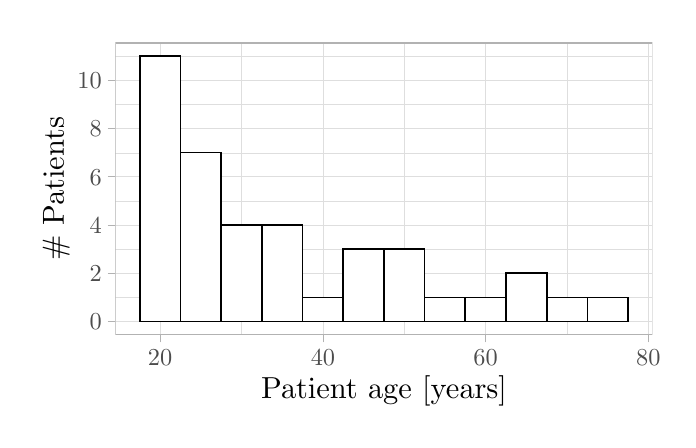
\begin{tikzpicture}[x=1pt,y=1pt]
\definecolor{fillColor}{RGB}{255,255,255}
\path[use as bounding box,fill=fillColor,fill opacity=0.00] (0,0) rectangle (231.26,141.65);
\begin{scope}
\path[clip] (  0.00,  0.00) rectangle (231.26,141.65);
\definecolor{drawColor}{RGB}{255,255,255}
\definecolor{fillColor}{RGB}{255,255,255}

\path[draw=drawColor,line width= 0.6pt,line join=round,line cap=round,fill=fillColor] (  0.00,  0.00) rectangle (231.26,141.65);
\end{scope}
\begin{scope}
\path[clip] ( 31.71, 30.69) rectangle (225.76,136.15);
\definecolor{fillColor}{RGB}{255,255,255}

\path[fill=fillColor] ( 31.71, 30.69) rectangle (225.76,136.15);
\definecolor{drawColor}{gray}{0.87}

\path[draw=drawColor,line width= 0.1pt,line join=round] ( 31.71, 44.20) --
	(225.76, 44.20);

\path[draw=drawColor,line width= 0.1pt,line join=round] ( 31.71, 61.63) --
	(225.76, 61.63);

\path[draw=drawColor,line width= 0.1pt,line join=round] ( 31.71, 79.06) --
	(225.76, 79.06);

\path[draw=drawColor,line width= 0.1pt,line join=round] ( 31.71, 96.49) --
	(225.76, 96.49);

\path[draw=drawColor,line width= 0.1pt,line join=round] ( 31.71,113.92) --
	(225.76,113.92);

\path[draw=drawColor,line width= 0.1pt,line join=round] ( 31.71,131.36) --
	(225.76,131.36);

\path[draw=drawColor,line width= 0.1pt,line join=round] ( 77.28, 30.69) --
	( 77.28,136.15);

\path[draw=drawColor,line width= 0.1pt,line join=round] (136.09, 30.69) --
	(136.09,136.15);

\path[draw=drawColor,line width= 0.1pt,line join=round] (194.89, 30.69) --
	(194.89,136.15);

\path[draw=drawColor,line width= 0.3pt,line join=round] ( 31.71, 35.48) --
	(225.76, 35.48);

\path[draw=drawColor,line width= 0.3pt,line join=round] ( 31.71, 52.91) --
	(225.76, 52.91);

\path[draw=drawColor,line width= 0.3pt,line join=round] ( 31.71, 70.34) --
	(225.76, 70.34);

\path[draw=drawColor,line width= 0.3pt,line join=round] ( 31.71, 87.78) --
	(225.76, 87.78);

\path[draw=drawColor,line width= 0.3pt,line join=round] ( 31.71,105.21) --
	(225.76,105.21);

\path[draw=drawColor,line width= 0.3pt,line join=round] ( 31.71,122.64) --
	(225.76,122.64);

\path[draw=drawColor,line width= 0.3pt,line join=round] ( 47.88, 30.69) --
	( 47.88,136.15);

\path[draw=drawColor,line width= 0.3pt,line join=round] (106.69, 30.69) --
	(106.69,136.15);

\path[draw=drawColor,line width= 0.3pt,line join=round] (165.49, 30.69) --
	(165.49,136.15);

\path[draw=drawColor,line width= 0.3pt,line join=round] (224.29, 30.69) --
	(224.29,136.15);
\definecolor{drawColor}{RGB}{0,0,0}

\path[draw=drawColor,line width= 0.6pt,line cap=rect,fill=fillColor] ( 40.53, 35.48) rectangle ( 55.23,131.36);

\path[draw=drawColor,line width= 0.6pt,line cap=rect,fill=fillColor] ( 55.23, 35.48) rectangle ( 69.93, 96.49);

\path[draw=drawColor,line width= 0.6pt,line cap=rect,fill=fillColor] ( 69.93, 35.48) rectangle ( 84.64, 70.34);

\path[draw=drawColor,line width= 0.6pt,line cap=rect,fill=fillColor] ( 84.64, 35.48) rectangle ( 99.34, 70.34);

\path[draw=drawColor,line width= 0.6pt,line cap=rect,fill=fillColor] ( 99.34, 35.48) rectangle (114.04, 44.20);

\path[draw=drawColor,line width= 0.6pt,line cap=rect,fill=fillColor] (114.04, 35.48) rectangle (128.74, 61.63);

\path[draw=drawColor,line width= 0.6pt,line cap=rect,fill=fillColor] (128.74, 35.48) rectangle (143.44, 61.63);

\path[draw=drawColor,line width= 0.6pt,line cap=rect,fill=fillColor] (143.44, 35.48) rectangle (158.14, 44.20);

\path[draw=drawColor,line width= 0.6pt,line cap=rect,fill=fillColor] (158.14, 35.48) rectangle (172.84, 44.20);

\path[draw=drawColor,line width= 0.6pt,line cap=rect,fill=fillColor] (172.84, 35.48) rectangle (187.54, 52.91);

\path[draw=drawColor,line width= 0.6pt,line cap=rect,fill=fillColor] (187.54, 35.48) rectangle (202.24, 44.20);

\path[draw=drawColor,line width= 0.6pt,line cap=rect,fill=fillColor] (202.24, 35.48) rectangle (216.94, 44.20);
\definecolor{drawColor}{gray}{0.70}

\path[draw=drawColor,line width= 0.6pt,line join=round,line cap=round] ( 31.71, 30.69) rectangle (225.76,136.15);
\end{scope}
\begin{scope}
\path[clip] (  0.00,  0.00) rectangle (231.26,141.65);
\definecolor{drawColor}{gray}{0.30}

\node[text=drawColor,anchor=base east,inner sep=0pt, outer sep=0pt, scale=  0.88] at ( 26.76, 32.45) {0};

\node[text=drawColor,anchor=base east,inner sep=0pt, outer sep=0pt, scale=  0.88] at ( 26.76, 49.88) {2};

\node[text=drawColor,anchor=base east,inner sep=0pt, outer sep=0pt, scale=  0.88] at ( 26.76, 67.31) {4};

\node[text=drawColor,anchor=base east,inner sep=0pt, outer sep=0pt, scale=  0.88] at ( 26.76, 84.75) {6};

\node[text=drawColor,anchor=base east,inner sep=0pt, outer sep=0pt, scale=  0.88] at ( 26.76,102.18) {8};

\node[text=drawColor,anchor=base east,inner sep=0pt, outer sep=0pt, scale=  0.88] at ( 26.76,119.61) {10};
\end{scope}
\begin{scope}
\path[clip] (  0.00,  0.00) rectangle (231.26,141.65);
\definecolor{drawColor}{gray}{0.70}

\path[draw=drawColor,line width= 0.3pt,line join=round] ( 28.96, 35.48) --
	( 31.71, 35.48);

\path[draw=drawColor,line width= 0.3pt,line join=round] ( 28.96, 52.91) --
	( 31.71, 52.91);

\path[draw=drawColor,line width= 0.3pt,line join=round] ( 28.96, 70.34) --
	( 31.71, 70.34);

\path[draw=drawColor,line width= 0.3pt,line join=round] ( 28.96, 87.78) --
	( 31.71, 87.78);

\path[draw=drawColor,line width= 0.3pt,line join=round] ( 28.96,105.21) --
	( 31.71,105.21);

\path[draw=drawColor,line width= 0.3pt,line join=round] ( 28.96,122.64) --
	( 31.71,122.64);
\end{scope}
\begin{scope}
\path[clip] (  0.00,  0.00) rectangle (231.26,141.65);
\definecolor{drawColor}{gray}{0.70}

\path[draw=drawColor,line width= 0.3pt,line join=round] ( 47.88, 27.94) --
	( 47.88, 30.69);

\path[draw=drawColor,line width= 0.3pt,line join=round] (106.69, 27.94) --
	(106.69, 30.69);

\path[draw=drawColor,line width= 0.3pt,line join=round] (165.49, 27.94) --
	(165.49, 30.69);

\path[draw=drawColor,line width= 0.3pt,line join=round] (224.29, 27.94) --
	(224.29, 30.69);
\end{scope}
\begin{scope}
\path[clip] (  0.00,  0.00) rectangle (231.26,141.65);
\definecolor{drawColor}{gray}{0.30}

\node[text=drawColor,anchor=base,inner sep=0pt, outer sep=0pt, scale=  0.88] at ( 47.88, 19.68) {20};

\node[text=drawColor,anchor=base,inner sep=0pt, outer sep=0pt, scale=  0.88] at (106.69, 19.68) {40};

\node[text=drawColor,anchor=base,inner sep=0pt, outer sep=0pt, scale=  0.88] at (165.49, 19.68) {60};

\node[text=drawColor,anchor=base,inner sep=0pt, outer sep=0pt, scale=  0.88] at (224.29, 19.68) {80};
\end{scope}
\begin{scope}
\path[clip] (  0.00,  0.00) rectangle (231.26,141.65);
\definecolor{drawColor}{RGB}{0,0,0}

\node[text=drawColor,anchor=base,inner sep=0pt, outer sep=0pt, scale=  1.10] at (128.74,  7.64) {Patient age [years]};
\end{scope}
\begin{scope}
\path[clip] (  0.00,  0.00) rectangle (231.26,141.65);
\definecolor{drawColor}{RGB}{0,0,0}

\node[text=drawColor,rotate= 90.00,anchor=base,inner sep=0pt, outer sep=0pt, scale=  1.10] at ( 13.08, 83.42) {\# Patients};
\end{scope}
\end{tikzpicture}

    }
    \begin{tabular}{@{\extracolsep{5pt}} cccccc} 
\\[-1.8ex]\hline 
\hline \\[-1.8ex] 
min & Q1 & median & mean & Q3 & max \\ 
\hline \\[-1.8ex] 
$19$ & $22$ & $30$ & $35$ & $43$ & $76$ \\ 
\hline \\[-1.8ex] 
\end{tabular} 
    \caption{Histogram of age distribution}
    \label{fig:agedist}
\end{figure}

